% Created 2016-07-27 周三 19:10
\documentclass[10pt,journal,onecolumn]{IEEEtran}
\usepackage[utf8]{inputenc}
\usepackage[T1]{fontenc}
\usepackage{fixltx2e}
\usepackage{graphicx}
\usepackage{longtable}
\usepackage{float}
\usepackage{wrapfig}
\usepackage{rotating}
\usepackage[normalem]{ulem}
\usepackage{amsmath}
\usepackage{textcomp}
\usepackage{marvosym}
\usepackage{wasysym}
\usepackage{amssymb}
\usepackage{hyperref}
\tolerance=1000
\usepackage{xeCJK}% 调用 xeCJK 宏包
\setCJKmainfont{SimSun}% 设置 CJK 主字体为 SimSun (宋体)
\date{}
\title{Kalman Filter 实战作业}
\hypersetup{
  pdfkeywords={},
  pdfsubject={},
  pdfcreator={Emacs 24.5.1 (Org mode 8.2.10)}}
\begin{document}

\maketitle
\section{引言}
\label{sec-1}
庆丰三年夏,董老师小讲kalman,谓吾等自行操练Kalman的formula,故有此记。
\section{初识Kalman}
\label{sec-2}
我研一已经看过了有关Kalman的books,只记得其时间更新以及状态更新的思想很深刻,过去两年后又有了新的感悟。在《Optimal State Estimation》一书中,作者是从递归最小二乘(RLS),很自然地过渡到Kalman Filter的。RLS产生的一个重要需求就是要递归估计,而不是batch mode,即:
\begin{IEEEeqnarray}{ll}
y_k&=H_kx_k+v_k \\
x_k&=\hat{x}_{k-1}+K_k(y_k-H_k\hat{x}_{k-1})
\end{IEEEeqnarray}
问题转化为如何求\(K_k\).

当然了,对于一个estimation任务,很自然的要先确定如何衡量这个estimation的好坏,而这个衡量标准(criterion)又可以作为我们的目标函数。在RLS中,如果将估计误差(即\(x-\hat{x}\))的期望\(E(\epsilon_{x,k})\)作为目标函数,对于零均值的测量噪声以及理想的状态初始值来说,则在对\(E(\epsilon_{x,k})\)进行递归估计时得不出什么重要信息(详见P84). 因此不得不另选一个目标函数,即估计误差的方差之和\(J_k=Trace(P_k)\)。通过简单的求导即可得到更新公式:
\begin{IEEEeqnarray}{ll}
K_k&=P_{k-1}H^T_k(H_kP_{k-1}H^T+R_k)^- \\
\hat{x}_k&=\hat{x}_{k-1}+K_k(y_k-H_k\hat{x}_{k-1}) \\
P_k&=(I-K_kH_k)P_{k-1}(I-K_kH_k)^T+K_kR_kK_k^T
\end{IEEEeqnarray}
当然,在RLS中,我们假定要估计的state是constant的。what if not? Then comes the Kalman Filter! 也就是说RLS中我们只有测量方程,现在需要考虑加入时间更新方程:
\begin{equation}
x_k=F_{k-1}x_{k-1}+G_{k-1}u_{k-1}+\omega_{k-1}
\end{equation}
此时更新公式只需要加入:(详见P128)
\begin{equation}
P_{k-1}=F_{k-1}P^1_{k-1}F_{k-1}^T+Q_{k-1}
\end{equation}
其中\(P^1_{k-1}\)即上一次测量更新得到的\(P_{k-1}\),这里为了和RLS的notation一致,加入了上标1.
现在回顾一下,RLS和Kalman的区别就是,在RLS中,直接令\(P_{k-1}=P^1_{k-1}\)(因为状态是恒定的嘛),在Kalman中加入了时间更新!这个更新是基于我们对这个system的dynamics的了解来的!
\section{Kalman for curve fitting(抛物线拟合)}
\label{sec-3}
我们认为其parameters,即states为\((a,b,c)\)恒定(实际上把Kalman当RLS来用啦),而测量方程为:
\begin{equation}
y[k]=ax[k]^2+bx[k]+c+w[k]
\end{equation}
每一次的测量相当于\([x[k]^2,x[k],1\mid y[k]]\).在code中,我们假设\((a,b,c)=(1, 2, 3)\),得到100组测量数据后,最终的estimate为\([ 1.00948328,1.95366774,3.04191686]\),每一次iteration的结果和error bar如下图所示(注,仅plot了第一个状态即\(a=1\)的estimation结果,其它两个类似就不画了)。
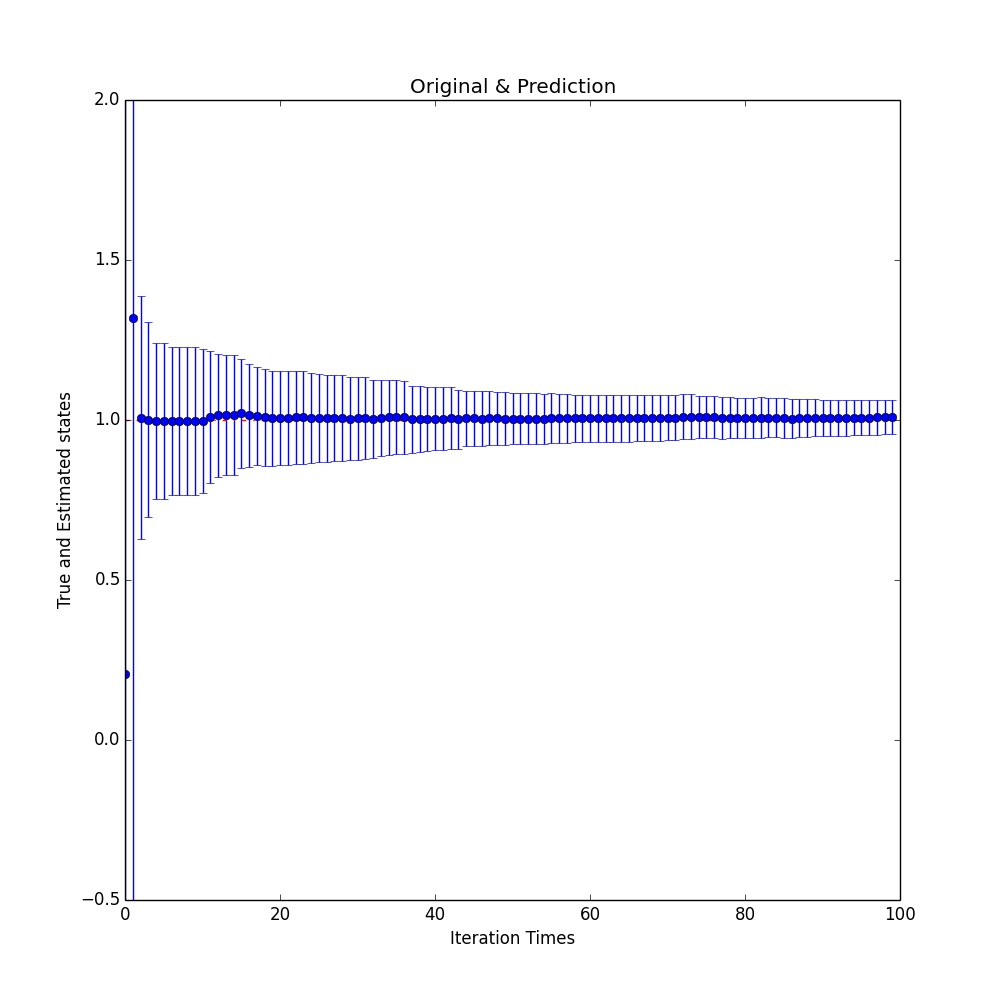
\includegraphics[width=3.5in]{kalman.jpeg}
\section{附录代码}
\label{sec-4}
注意第33行只是简单地将协方差矩阵进行传播,并没有使用时间更新方程。
\begin{verbatim}
 1  # coding=utf-8
 2  import matplotlib.pyplot as plt
 3  import numpy as np
 4  def kalman(A, y):
 5      """
 6      Formulars from the book《Optimal State Estimation》
 7      Page88 & P128
 8      :param A: array in the sklearn form. each "row"
 9       represents an input (the measurement coeffcient).
10      :param y:vector of the response variable (measuremen)
11      :return: x:the estimates. p: covariance of x
12      """
13      dim = A.shape[1]
14      n = A.shape[0]
15      # initialize the estimate of the state(s)
16      # and its(their) covirance
17      x0 = np.zeros((dim, 1))
18      P0 = 1e5 * np.identity(dim)
19      R = 1  # the measurement variance
20      # convert numpy arrays to matrix(suitable for matrix manupulation)
21      x0 = np.mat(x0)
22      P0 = np.mat(P0)
23      # start iteration
24      x, p = [], []
25      for i in range(n):
26          Hk = np.mat(A[i, :][:, np.newaxis]).T
27          Kk = P0 * Hk.T * (Hk * P0 * Hk.T + R).I
28          x_new = x0 + Kk * (y[i] - Hk * x0)
29          Pk = (np.mat(np.identity(dim)) - Kk * Hk) * P0 * \
30               (np.mat(np.identity(dim)) - Kk * Hk).T + Kk * R * Kk.T
31          #Note! this is not universal! We assume that the "time update"
32          #step is trival, i.e., the states are constants
33          #Modify the following line as you need.
34          P0 = Pk                                
35          x0 = x_new
36          # for return
37          x.append(x0)
38          p.append(P0)
39      #convert x back to array
40      x=[np.array(xi).squeeze() for xi in x]
41      return x,p
42  def testKalman():
43      #prepare training data (3-dimension)
44      dataLen = 100
45      A = np.random.random_sample((dataLen, 1)) * 5
46      A = np.c_[A ** 2, A, np.ones((dataLen, 1))]
47      x = np.array([1, 2, 3])
48      y = np.dot(A, x) + np.random.randn(dataLen) * 0.1
49      x_,p= kalman(A, y)
50      print "final estimate:",x_[-1]
51      #extract the confidence interval of the 0th state
52      y_err=[np.sqrt(pi[0,0]) for pi in p]
53      #now plot!
54      fig, ax = plt.subplots(1,1,figsize=(10,10))
55      ax.plot(range(dataLen),np.ones(dataLen)*x[0], 'r-.')
56      # ax.plot(range(dataLen),[xi[0] for xi in x_], 'b-x', alpha=0.5)
57      ax.errorbar(range(dataLen),[xi[0] for xi in x_], yerr=y_err, fmt='o')
58      ax.set_ylim([-0.5,2])
59      ax.set_title('Original & Prediction')
60      ax.set_xlabel(u'Iteration Times')
61      ax.set_ylabel(u'True and Estimated states')
62      plt.show()
63      pass
64  if __name__ == '__main__':
65      testKalman()
\end{verbatim}
% Emacs 24.5.1 (Org mode 8.2.10)
\end{document}
